\begin{enumerate}
    \item[8.] Encuentra las soluciones de equilibrio, di de que tipo son y haz un boceto de las soluciones a la ecuación autónoma.
\end{enumerate}
%\begin{align*}
%    y' = 5y^{2}-y^{3}+6y
%\end{align*}
%\begin{align*}
%    y' = 4y^{4}+4y^{3}-3y^{2}
%\end{align*}


\begin{itemize}
    \item[a)] $y'=5y^2-y^3+6y$
    \begin{enumerate}
        \item Primero factorizamos para encontrar las raíces.
        \begin{align*}
            5y^2-y^3+6y &= 0 \\
            -y(y^2-5y-6) &= 0 \\
            -y(y+1)(y-6) &= 0
        \end{align*}
        Entonces las raíces son:\hspace{.5cm} $y=0$\hspace{.5cm}$y=-1$\hspace{.5cm} $y=6$\\
        Las cuales son las soluciones de equilibrio de nuestra función.
        
        \item  Evaluamos en los alrededores de nuestras soluciones de equilibrio para observar como se comporta la derivada en esos puntos, y ver si son positivas o negativas.
        \begin{align*}
            f(7) &= 5(7)^2 -(7)^3+6(7) =-56 < 0\\
            f(5) &= 30 > 0\\
            f(1) &= 10 > 0 \\
            f(-2) &= 16 > 0
        \end{align*}
        Y así podemos realizar nuestro boceto donde vemos que tipo de punto son las soluciones de equilibrio.
        \item Boceto y tipos de soluciones de equilibrio
\begin{figure}[H]
    \centering
    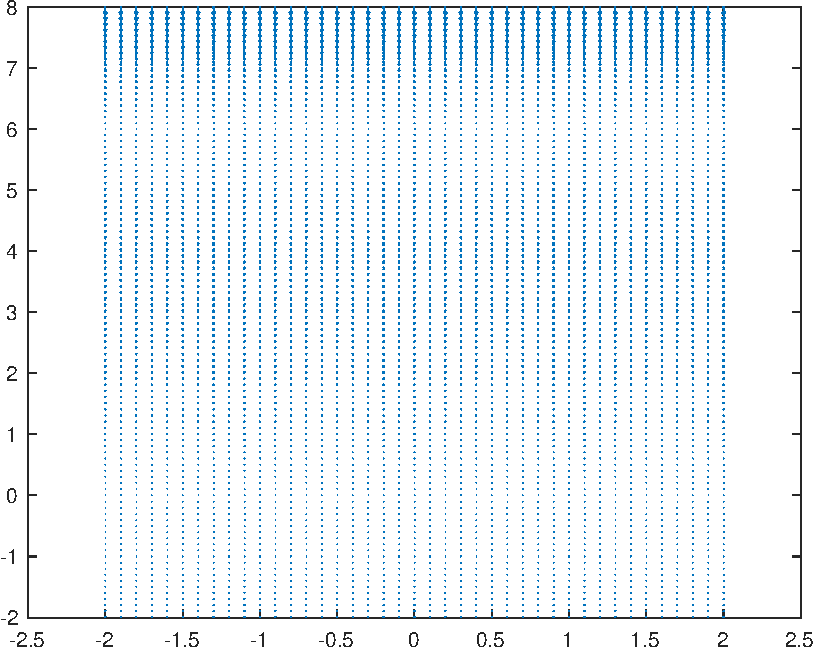
\includegraphics[scale=.8]{IM/B2.pdf}
    \caption{Boceto 1}
    \label{fig=int1}
\end{figure}
        
        Como podemos observar en el boceto de las soluciones $y=6 $ es un punto estable.
\end{enumerate}

\item[b)] $y'=4y^4+4y^3-3y^2$
\begin{enumerate}
    \item Primero factorizamos para encontrar las raíces.
    \begin{align*}
        4y^4+4y^3-3y^2 &= 0 \\
        y^2(4y^2+4y-3) &= 0 \\
        y^2(2y+3)(2y-1) &= 0
    \end{align*}
    Entonces las raíces son:\hspace{.5cm} $y=0$\hspace{.5cm}$y=-\frac{3}{2}$\hspace{.5cm} $y=\frac{1}{2}$\\
        Las cuales son las soluciones de equilibrio de nuestra función.
    \item  Evaluamos en los alrededores de nuestras soluciones de equilibrio para observar como se comporta la derivada en esos puntos, y ver si son positivas o negativas.
    \begin{align*}
        f(1) &= 4(1)^4+4(1)^3-3(1)^2  = 5 > 0\\
        f(\frac{1}{4}) &= -\frac{7}{64} < 0\\
        f(-\frac{1}{2}) &= -1 < 0 \\
        f(-1) &= -3 < 0\\
        f(-2) &= 20 > 0
    \end{align*}
        Y así podemos realizar nuestro boceto donde vemos que tipo de punto son las soluciones de equilibrio.
        \item Boceto y tipos de soluciones de equilibrio
\begin{figure}[H]
    \centering
    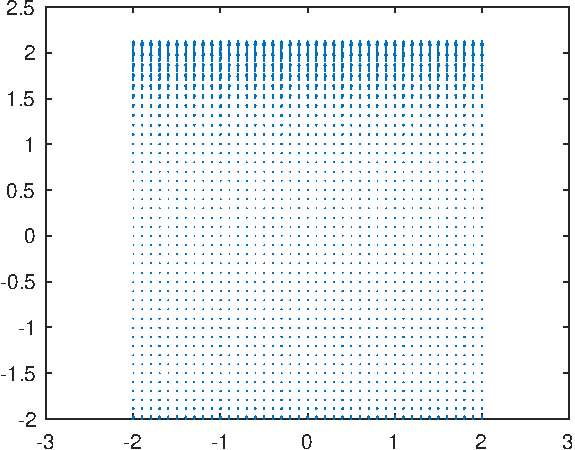
\includegraphics[scale=1.2]{IM/b1.pdf}
    \caption{Boceto 2}
    \label{fig=int1}
\end{figure}
        Como podemos observar en el boceto de las soluciones $y=\frac{1}{2}$ es un punto inestable y $y=-\frac{3}{2}$ es un punto estable.
    
\end{enumerate}

\end{itemize}
